\documentclass{fancyslides} 
\usepackage[utf8]{inputenc}
\usepackage{times}
\usepackage{algorithm2e}
\usepackage{listings}
\usepackage{hyperref}


%%% Beamer settings (do not change)
\usetheme{default} 
\setbeamertemplate{navigation symbols}{} %no navigation symbols
\setbeamercolor{structure}{fg=\yourowntexcol} 
\setbeamercolor{normal text}{fg=\yourowntexcol} 



%%%%%%%%%%%%%%%%%%%%%%%%%
%%% CUSTOMISATIONS %%%%%%
%%%%%%%%%%%%%%%%%%%%%%%%%

% THE FOLLOWING COLOURS ARE PREDEFINED IN THE CLASS
%bi -- WHITE
%cz -- BLACK
%sz -- GRAY
%nieb -- BLUE
%ziel -- GREEN
%pom -- ORANGE
%% YOU CAN DEFINE YOUR OWN COLOUR TO USE HERE. SEE MAN.PDF


%%%% SLIDE ELEMENTS
\newcommand{\structureopacity}{0.75} %opacity for the structure elements (boxes and dots)
\newcommand{\strcolor}{ziel} %elements colour (predefined nieb; pom; ziel)

%%%% TEXT COLOUR
\newcommand{\yourowntexcol}{bi}
\newcommand{\stext}[1]{{\color{black}#1}}
\newcommand{\ctext}[1]{{\ttfamily#1}}



%%%%%%%%%%%%%%%%%%%%%%%%%
%%% TITLE SLIDE DATA %%%%
%%%%%%%%%%%%%%%%%%%%%%%%%
\newcommand{\titlephrase}{Mesh Processing with OpenMesh and C++}
\newcommand{\name}{Alexandre Kaspar}
\newcommand{\affil}{EPFL / MIT}
\newcommand{\email}{akaspar@mit.edu}

\begin{document}

%\fontencoding{T1}
%\fontfamily{serif}
%\fontseries{m}
%\fontshape{it}
%\fontsize{12}{15}
%\selectfont

\lstset{
	language=C++,
    basicstyle=\color{black}\ttfamily,
    keywordstyle=\color{blue},
    identifierstyle=\color{gray!50!black},
    stringstyle=\color{green!50!black},
    commentstyle=\color{gray}\ttfamily\textit,
    morecomment=[l][\color{magenta}]{\#},
    numbers=left,
    numberstyle=\ttfamily,
    numbersep=10pt,
    xleftmargin=1cm
}

\setbeamercolor{frametitle}{fg=gray}

\startingslide %this generates titlepage from the data above

%%%%%%%%%%%%%%%%%%%%%%%%%
%%% SLIDES %%%%%%%%%%%%%%
%%%%%%%%%%%%%%%%%%%%%%%%%


%%%%%%%%%%%%%%%%%%%%%%%%%%%%%%%%%%%%%%%%%%%%%%%%%%%%%%%%%%%%%%%%%%%%%%%%%%%%%
%%%%% Hello world %%%%%%%%%%%%%%%%%%%%%%%%%%%%%%%%%%%%%%%%%%%%%%%%%%%%%%%%%%%
%%%%%%%%%%%%%%%%%%%%%%%%%%%%%%%%%%%%%%%%%%%%%%%%%%%%%%%%%%%%%%%%%%%%%%%%%%%%%
\begin{frame}
\pointedsl{Hello World!}
\end{frame}

\begin{frame}[fragile]
\frametitle{Hello World}
\begin{lstlisting}
#include<iostream>
// A comment
int main(int argc, char **argv){
    std::cout << "Hello world!\n";
    return 0;
}
\end{lstlisting}
\misc{
	Outputs "Hello world!" to the console and exits.
}
\end{frame}

%%%%%%%%%%%%%%%%%%%%%%%%%%%%%%%%%%%%%%%%%%%%%%%%%%%%%%%%%%%%%%%%%%%%%%%%%%%%%
%%%%% Pre-processor %%%%%%%%%%%%%%%%%%%%%%%%%%%%%%%%%%%%%%%%%%%%%%%%%%%%%%%%%
%%%%%%%%%%%%%%%%%%%%%%%%%%%%%%%%%%%%%%%%%%%%%%%%%%%%%%%%%%%%%%%%%%%%%%%%%%%%%
\begin{frame}[fragile]
\frametitle{Pre-processor instructions}
\begin{lstlisting}
#include<iostream>
\end{lstlisting}
\misc{
	Lines starting with a `\#' (pound) are instructions parsed by the \emph{pre-processor} such as
	\begin{itemize}
	\item \textbf{\#include} specifies a file to be included at this line.
	\item \textbf{\#if, \#ifdef, \#endif} conditionally uses a block of code.
	\item \textbf{\#define} creates an alias for an expression.
	\end{itemize}
}
\end{frame}

%%%%%%%%%%%%%%%%%%%%%%%%%%%%%%%%%%%%%%%%%%%%%%%%%%%%%%%%%%%%%%%%%%%%%%%%%%%%%
%%%%% Comments %%%%%%%%%%%%%%%%%%%%%%%%%%%%%%%%%%%%%%%%%%%%%%%%%%%%%%%%%%%%%%
%%%%%%%%%%%%%%%%%%%%%%%%%%%%%%%%%%%%%%%%%%%%%%%%%%%%%%%%%%%%%%%%%%%%%%%%%%%%%
\begin{frame}[fragile]
\frametitle{Comments}
\begin{lstlisting}[firstnumber=2]
// A comment (up to the end of the line)
\end{lstlisting}
\stext{or}
\begin{lstlisting}[firstnumber=2]
/* A comment 
possibly spanning
multiple lines */
\end{lstlisting}
\misc{
	are two types of comments, which the compiler ignores.
}
\end{frame}

%%%%%%%%%%%%%%%%%%%%%%%%%%%%%%%%%%%%%%%%%%%%%%%%%%%%%%%%%%%%%%%%%%%%%%%%%%%%%
%%%%% Main function %%%%%%%%%%%%%%%%%%%%%%%%%%%%%%%%%%%%%%%%%%%%%%%%%%%%%%%%%
%%%%%%%%%%%%%%%%%%%%%%%%%%%%%%%%%%%%%%%%%%%%%%%%%%%%%%%%%%%%%%%%%%%%%%%%%%%%%
\begin{frame}[fragile]
\frametitle{Main function}
\begin{lstlisting}[firstnumber=3]
int main(int argc, char **argv){
    ...
    return 0;
}
\end{lstlisting}
\misc{
	defines a function named \ctext{main} which
	\begin{itemize}
		\item takes two arguments \ctext{argc} and \ctext{argv},
		\item returns an integer value (\ctext{int} in front).
	\end{itemize}
	\phantom{.}
}
\end{frame}

\begin{frame}[fragile]
\frametitle{Main function (2)}
\begin{lstlisting}[firstnumber=3]
int main(int argc, char **argv){
    ...
    return 0;
}
\end{lstlisting}
\misc{
	The \ctext{main} function is called when the program starts, with
	\begin{itemize}
		\item \ctext{argc}, the number of arguments
		\item \ctext{argv}, the arguments (array of strings)
	\end{itemize}
	and returns an integer code ($0=$ success).
}
\end{frame}

%%%%%%%%%%%%%%%%%%%%%%%%%%%%%%%%%%%%%%%%%%%%%%%%%%%%%%%%%%%%%%%%%%%%%%%%%%%%%
%%%%% Output statement %%%%%%%%%%%%%%%%%%%%%%%%%%%%%%%%%%%%%%%%%%%%%%%%%%%%%%
%%%%%%%%%%%%%%%%%%%%%%%%%%%%%%%%%%%%%%%%%%%%%%%%%%%%%%%%%%%%%%%%%%%%%%%%%%%%%
\begin{frame}[fragile]
\frametitle{Output statement}
\begin{lstlisting}[firstnumber=4]
std::cout << "Hello world!\n";
\end{lstlisting}
\misc{
\begin{itemize}
	\item \ctext{std} is the standard \emph{namespace}.
	\item \ctext{cout} is a \emph{Stream} object.
	\item \ctext{<<} is the output operator of \emph{Stream}.
	\item \ctext{"Hello world"} is the string being output.
\end{itemize}
}
\end{frame}

%%%%%%%%%%%%%%%%%%%%%%%%%%%%%%%%%%%%%%%%%%%%%%%%%%%%%%%%%%%%%%%%%%%%%%%%%%%%%
%%%%% Basic C++ %%%%%%%%%%%%%%%%%%%%%%%%%%%%%%%%%%%%%%%%%%%%%%%%%%%%%%%%%%%%%
%%%%%%%%%%%%%%%%%%%%%%%%%%%%%%%%%%%%%%%%%%%%%%%%%%%%%%%%%%%%%%%%%%%%%%%%%%%%%
\begin{frame}
\pointedsl{
	Basics
}
\end{frame}

%%%%%%%%%%%%%%%%%%%%%%%%%%%%%%%%%%%%%%%%%%%%%%%%%%%%%%%%%%%%%%%%%%%%%%%%%%%%%
\lstset{language=C++,numbers=none}
\begin{frame}[fragile]
\frametitle{Declaration and definition}
\begin{lstlisting}
void process(int x); // declare a function
int x; // declare a variable
x = 10; // assign a value
process(x);
// declaration and definition
int sum(int a, int b){ return a + b; }
// declaration and assignment
int y = sum(x, 2);
\end{lstlisting}
\misc{
	Every variable, type or function must be declared before being used. They can then be defined anywhere.
	
	\textbf{Note}: variables automatically receive a default value corresponding to $0$.
}
\end{frame}

%%%%%%%%%%%%%%%%%%%%%%%%%%%%%%%%%%%%%%%%%%%%%%%%%%%%%%%%%%%%%%%%%%%%%%%%%%%%%
\begin{frame}[fragile]
\frametitle{Flow control}
\begin{center}
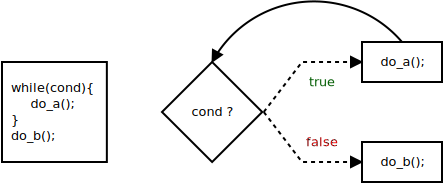
\includegraphics[width=0.7\textwidth]{figures/flow}
\end{center}
\misc{
	The usual conditional blocks are available
	\begin{itemize}
		\item \ctext{if}, \ctext{else if}, \ctext{else} and \ctext{switch}
	\end{itemize}
	as well as loop structures
	\begin{itemize}
		\item \ctext{for}, \ctext{while} and \ctext{do while}
	\end{itemize}
}
\end{frame}

%%%%%%%%%%%%%%%%%%%%%%%%%%%%%%%%%%%%%%%%%%%%%%%%%%%%%%%%%%%%%%%%%%%%%%%%%%%%%
\begin{frame}[fragile]
\frametitle{Arrays}
\begin{columns}[c]
  \begin{column}{0.5\textwidth}
\lstset{language=C++,numbers=left}
\begin{lstlisting}
int a[3] = { 1, 0 };
a[1] = 42;
// a[2] == 0
\end{lstlisting}
  \end{column}
  \begin{column}{0.5\textwidth}
    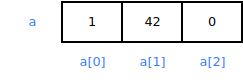
\includegraphics[width=0.95\textwidth]{figures/array0}
  \end{column}
\end{columns}
\misc{
	\emph{Arrays} are continuous blocks of memory that store multiple elements of a same type. They use $0$-based indexing.
}
\end{frame}


%%%%%%%%%%%%%%%%%%%%%%%%%%%%%%%%%%%%%%%%%%%%%%%%%%%%%%%%%%%%%%%%%%%%%%%%%%%%%
%%%%% Advanced C++ %%%%%%%%%%%%%%%%%%%%%%%%%%%%%%%%%%%%%%%%%%%%%%%%%%%%%%%%%%
%%%%%%%%%%%%%%%%%%%%%%%%%%%%%%%%%%%%%%%%%%%%%%%%%%%%%%%%%%%%%%%%%%%%%%%%%%%%%
\begin{frame}
\pointedsl{
	Advanced C++
}
\end{frame}

%%%%%%%%%%%%%%%%%%%%%%%%%%%%%%%%%%%%%%%%%%%%%%%%%%%%%%%%%%%%%%%%%%%%%%%%%%%%%
\begin{frame}[fragile]
\frametitle{References}
\begin{lstlisting}
// passed by reference
void swap_ref(int &x, int &y){
    int tmp = x;
    x = y;
    y = tmp;
}
int a = 1, b = 2;
swap_ref(a, b);
// good! a=2, b=1
\end{lstlisting}
\misc{
	\emph{References} are syntactic sugar for pointers when passing variables to functions or retrieving the value they return.
}
\end{frame}

%%%%%%%%%%%%%%%%%%%%%%%%%%%%%%%%%%%%%%%%%%%%%%%%%%%%%%%%%%%%%%%%%%%%%%%%%%%%%
\begin{frame}[fragile]
\frametitle{Templating}
\begin{lstlisting}
template< typename T >
T sum(T a, T b){
    T c = a + b;
    return c;
}
\end{lstlisting}
\misc{
	Function (and class) \emph{templates} provides a way to abstract the notion of type.
	
	Here, the type \ctext{T} is resolved by the compiler when \ctext{sum} is used.
	It only requires an operator \ctext{+} to work.
}
\end{frame}

%%%%%%%%%%%%%%%%%%%%%%%%%%%%%%%%%%%%%%%%%%%%%%%%%%%%%%%%%%%%%%%%%%%%%%%%%%%%%
\begin{frame}[fragile]
\frametitle{Templating (2)}
\begin{lstlisting}
int c = sum(1, 2);
float d = sum(1.0f, 2.0f);
float e = sum<float>(1, 2.0f);
\end{lstlisting}
\misc{
	The type \ctext{T} can sometimes by inferred. When it cannot, one must specify it.
}
\end{frame}

%%%%%%%%%%%%%%%%%%%%%%%%%%%%%%%%%%%%%%%%%%%%%%%%%%%%%%%%%%%%%%%%%%%%%%%%%%%%%
\begin{frame}[fragile]
\frametitle{Classes}
\begin{lstlisting}
// declaration
template <typename T, int dim>
struct vec {
    typedef vec<T, dim> this_type;
    T val[dim];
    vec(T a, T b);
    double sqLength() const;
    static this_type constant(T a);
};
\end{lstlisting}
\misc{
	Classes (keyword \ctext{class}) and structures (keyword \ctext{struct}) describe custom types made
	of properties (\ctext{val}) and methods (\ctext{sqLength}).
}
\end{frame}

\begin{frame}[fragile]
\frametitle{Classes (2)}
\begin{lstlisting}
// definitions
template <typename T, int dim>
double vec<T, dim>::sqLength() {
    T sum = 0;
    for(int i = 0; i < dim; ++i)
        sum += val[i] * val[i];
    return sum;
}
\end{lstlisting}
\misc{
	Definition of methods (including the constructor \ctext{vec} and/or its possible destructor \ctext{~vec} can be done separately.
}
\end{frame}

\begin{frame}[fragile]
\frametitle{Classes (3)}
\begin{lstlisting}
// type alias
typedef vec<float, 2> vec2f;

// class usage
vec2f a = vec2f::constant(2);
float d = a.sqLength(); // d=8
\end{lstlisting}
\misc{
	Static properties and methods are called with the namespace operator (\ctext{::}) whereas
	instance properties and methods are accessed with the dot operator.
}
\end{frame}

\begin{frame}[fragile]
\frametitle{Operator overloading}
\begin{lstlisting}
vec2f operator +(const vec2f &v1,
                 const vec2f &v2){
    vec2f x;
    for(int i = 0; i < 2; ++i)
        x.val[i] = v1.val[i] + v2.val[i];
    return x;
}

// usage
vec2f a, b;
// hidden: initialization of a and b
vec3f c = a + b;
\end{lstlisting}
\end{frame}


%%%%%%%%%%%%%%%%%%%%%%%%%%%%%%%%%%%%%%%%%%%%%%%%%%%%%%%%%%%%%%%%%%%%%%%%%%%%%
%%%%% C++ and Memory %%%%%%%%%%%%%%%%%%%%%%%%%%%%%%%%%%%%%%%%%%%%%%%%%%%%%%%%
%%%%%%%%%%%%%%%%%%%%%%%%%%%%%%%%%%%%%%%%%%%%%%%%%%%%%%%%%%%%%%%%%%%%%%%%%%%%%
\begin{frame}
\pointedsl{
	Stack / Heap
}
\end{frame}

% See http://stackoverflow.com/questions/79923/what-and-where-are-the-stack-and-heap
% See http://gribblelab.org/CBootcamp/7_Memory_Stack_vs_Heap.html
% See http://www.learncpp.com/cpp-tutorial/79-the-stack-and-the-heap/

%%%%%%%%%%%%%%%%%%%%%%%%%%%%%%%%%%%%%%%%%%%%%%%%%%%%%%%%%%%%%%%%%%%%%%%%%%%%%
\begin{frame}[fragile]
\frametitle{References}
\begin{lstlisting}
// passed by reference
void swap_ref(int &x, int &y){
    int tmp = x;
    x = y;
    y = tmp;
}
int a = 1, b = 2;
swap_ref(a, b);
// good! a=2, b=1
\end{lstlisting}
\misc{
	\emph{References} are syntactic sugar for pointers when passing variables to functions or retrieving the value they return.
}
\end{frame}


%%%%%%%%%%%%%%%%%%%%%%%%%%%%%%%%%%%%%%%%%%%%%%%%%%%%%%%%%%%%%%%%%%%%%%%%%%%%%
%%%%% CPP %%%%%%%%%%%%%%%%%%%%%%%%%%%%%%%%%%%%%%%%%%%%%%%%%%%%%%%%%%%%%%%%%%%
%%%%%%%%%%%%%%%%%%%%%%%%%%%%%%%%%%%%%%%%%%%%%%%%%%%%%%%%%%%%%%%%%%%%%%%%%%%%%

\fbckg{backgrounds/3dparis2}
\begin{frame}
\pointedsl{OpenMesh}
\end{frame}

\setbeamercolor{frametitle}{fg=white}

\begin{frame}
\frametitle{OpenMesh}
\itemized{
	\item C++ library to work with polygonal meshes
	\item Half-edge data structure
	\item Efficient and flexible
}
\end{frame}

\setbeamercolor{frametitle}{fg=gray}

% based on http://www.openmesh.org/media/Documentations/OpenMesh-Doc-Latest/a00012.html


%%%%%%%%%%%%%%%%%%%%%%%%%
%%% ENDING %%%%%%%%%%%%%%
%%%%%%%%%%%%%%%%%%%%%%%%%

\fbckg{backgrounds/blank2}
\begin{frame}
  \thankyou   %%%% ending slide with thank you notice
\end{frame}

\begin{frame}
\sources{

\includegraphics[height=1em]{figures/C++-logo} \ \href{http://ocw.mit.edu/courses/electrical-engineering-and-computer-science/6-096-introduction-to-c-january-iap-2011/index.htm}{Introduction to C++,  MIT OpenCourseWare}\\

\includegraphics[height=1em]{figures/C++-logo} \ \url{http://www.openmesh.org}
}
\end{frame}


\end{document}